% !TeX TXS-program:bibliography = txs:///biber
\documentclass[14pt, russian]{scrartcl}
\let\counterwithout\relax
\let\counterwithin\relax
%\usepackage{lmodern}
\usepackage{float}
\usepackage{xcolor}
\usepackage{extsizes}
\usepackage{subfig}
\usepackage[export]{adjustbox}
\usepackage{tocvsec2} % возможность менять учитываемую глубину разделов в оглавлении
\usepackage[subfigure]{tocloft}
\usepackage[newfloat,outputdir=build]{minted}
\captionsetup[listing]{position=top}

\AtBeginEnvironment{figure}{\vspace{0.5cm}}
\AtBeginEnvironment{table}{\vspace{0.5cm}}
\AtBeginEnvironment{listing}{\vspace{0.5cm}}
\AtBeginEnvironment{algorithm}{\vspace{0.5cm}}
\AtBeginEnvironment{minted}{\vspace{-0.5cm}}

\usepackage{fancyvrb}
\usepackage{ulem,bm,mathrsfs,ifsym} %зачеркивания, особо жирный стиль и RSFS начертание
\usepackage{sectsty} % переопределение стилей подразделов
%%%%%%%%%%%%%%%%%%%%%%%

%%% Поля и разметка страницы %%%
\usepackage{pdflscape}                              % Для включения альбомных страниц
\usepackage{geometry}                               % Для последующего задания полей
\geometry{a4paper,tmargin=2cm,bmargin=2cm,lmargin=3cm,rmargin=1cm} % тоже самое, но лучше

%%% Математические пакеты %%%
\usepackage{amsthm,amsfonts,amsmath,amssymb,amscd}  % Математические дополнения от AMS
\usepackage{mathtools}                              % Добавляет окружение multlined
\usepackage[perpage]{footmisc}
%\usepackage{times}

%%%% Установки для размера шрифта 14 pt %%%%
%% Формирование переменных и констант для сравнения (один раз для всех подключаемых файлов)%%
%% должно располагаться до вызова пакета fontspec или polyglossia, потому что они сбивают его работу
%\newlength{\curtextsize}
%\newlength{\bigtextsize}
%\setlength{\bigtextsize}{13pt}
\KOMAoptions{fontsize=14pt}

\makeatletter
\def\showfontsize{\f@size{} point}
\makeatother

%\makeatletter
%\show\f@size                                       % неплохо для отслеживания, но вызывает стопорение процесса, если документ компилируется без команды  -interaction=nonstopmode
%\setlength{\curtextsize}{\f@size pt}
%\makeatother

%шрифт times
\usepackage{tempora}
%\usepackage{pscyr}
%\setmainfont[Ligatures={TeX,Historic}]{Times New Roman}

   %%% Решение проблемы копирования текста в буфер кракозябрами
%    \input glyphtounicode.tex
%    \input glyphtounicode-cmr.tex %from pdfx package
%    \pdfgentounicode=1
    \usepackage{cmap}                               % Улучшенный поиск русских слов в полученном pdf-файле
    \usepackage[T1]{fontenc}                       % Поддержка русских букв
    \usepackage[utf8]{inputenc}                     % Кодировка utf8
    \usepackage[english, main=russian]{babel}            % Языки: русский, английский
%   \IfFileExists{pscyr.sty}{\usepackage{pscyr}}{}  % Красивые русские шрифты
%\renewcommand{\rmdefault}{ftm}
%%% Оформление абзацев %%%
\usepackage{indentfirst}                            % Красная строка
%\usepackage{eskdpz}

%%% Таблицы %%%
\usepackage{longtable}                              % Длинные таблицы
\usepackage{multirow,makecell,array}                % Улучшенное форматирование таблиц
\usepackage{booktabs}                               % Возможность оформления таблиц в классическом книжном стиле (при правильном использовании не противоречит ГОСТ)

%%% Общее форматирование
\usepackage{soulutf8}                               % Поддержка переносоустойчивых подчёркиваний и зачёркиваний
\usepackage{icomma}                                 % Запятая в десятичных дробях



%%% Изображения %%%
\usepackage{graphicx}                               % Подключаем пакет работы с графикой
\usepackage{wrapfig}

\usepackage{tikz}
\usetikzlibrary{shapes.misc}
\usetikzlibrary{trees}

%%% Списки %%%
\usepackage{enumitem}

%%% Подписи %%%
\usepackage{caption}                                % Для управления подписями (рисунков и таблиц) % Может управлять номерами рисунков и таблиц с caption %Иногда может управлять заголовками в списках рисунков и таблиц
%% Использование:
%\begin{table}[h!]\ContinuedFloat - чтобы не переключать счетчик
%\captionsetup{labelformat=continued}% должен стоять до самого caption
%\caption{}
% либо ручками \caption*{Продолжение таблицы~\ref{...}.} :)

%%% Интервалы %%%
\addto\captionsrussian{%
  \renewcommand{\listingname}{Листинг}%
}
%%% Счётчики %%%
\usepackage[figure,table,section]{totalcount}               % Счётчик рисунков и таблиц
\DeclareTotalCounter{lstlisting}
\usepackage{totcount}                               % Пакет создания счётчиков на основе последнего номера подсчитываемого элемента (может требовать дважды компилировать документ)
\usepackage{totpages}                               % Счётчик страниц, совместимый с hyperref (ссылается на номер последней страницы). Желательно ставить последним пакетом в преамбуле

%%% Продвинутое управление групповыми ссылками (пока только формулами) %%%
%% Кодировки и шрифты %%%

%   \newfontfamily{\cyrillicfont}{Times New Roman}
%   \newfontfamily{\cyrillicfonttt}{CMU Typewriter Text}
	%\setmainfont{Times New Roman}
	%\newfontfamily\cyrillicfont{Times New Roman}
	%\setsansfont{Times New Roman}                    %% задаёт шрифт без засечек
%	\setmonofont{Liberation Mono}               %% задаёт моноширинный шрифт
%    \IfFileExists{pscyr.sty}{\renewcommand{\rmdefault}{ftm}}{}
%%% Интервалы %%%
%linespread-реализация ближе к реализации полуторного интервала в ворде.
%setspace реализация заточена под шрифты 10, 11, 12pt, под остальные кегли хуже, но всё же ближе к типографской классике.
\linespread{1.3}                    % Полуторный интервал (ГОСТ Р 7.0.11-2011, 5.3.6)
%\renewcommand{\@biblabel}[1]{#1}

%%% Гиперссылки %%%
\usepackage{hyperref}

%%% Выравнивание и переносы %%%
\sloppy                             % Избавляемся от переполнений
\clubpenalty=10000                  % Запрещаем разрыв страницы после первой строки абзаца
\widowpenalty=10000                 % Запрещаем разрыв страницы после последней строки абзаца

\makeatletter % малые заглавные, small caps shape
\let\@@scshape=\scshape
\renewcommand{\scshape}{%
  \ifnum\strcmp{\f@series}{bx}=\z@
    \usefont{T1}{cmr}{bx}{sc}%
  \else
    \ifnum\strcmp{\f@shape}{it}=\z@
      \fontshape{scsl}\selectfont
    \else
      \@@scshape
    \fi
  \fi}
\makeatother

%%% Подписи %%%
%\captionsetup{%
%singlelinecheck=off,                % Многострочные подписи, например у таблиц
%skip=2pt,                           % Вертикальная отбивка между подписью и содержимым рисунка или таблицы определяется ключом
%justification=centering,            % Центрирование подписей, заданных командой \caption
%}
%%%        Подключение пакетов                 %%%
\usepackage{ifthen}                 % добавляет ifthenelse
%%% Инициализирование переменных, не трогать!  %%%
\newcounter{intvl}
\newcounter{otstup}
\newcounter{contnumeq}
\newcounter{contnumfig}
\newcounter{contnumtab}
\newcounter{pgnum}
\newcounter{bibliosel}
\newcounter{chapstyle}
\newcounter{headingdelim}
\newcounter{headingalign}
\newcounter{headingsize}
\newcounter{tabcap}
\newcounter{tablaba}
\newcounter{tabtita}
%%%%%%%%%%%%%%%%%%%%%%%%%%%%%%%%%%%%%%%%%%%%%%%%%%

%%% Область упрощённого управления оформлением %%%

%% Интервал между заголовками и между заголовком и текстом
% Заголовки отделяют от текста сверху и снизу тремя интервалами (ГОСТ Р 7.0.11-2011, 5.3.5)
\setcounter{intvl}{3}               % Коэффициент кратности к размеру шрифта

%% Отступы у заголовков в тексте
\setcounter{otstup}{0}              % 0 --- без отступа; 1 --- абзацный отступ

%% Нумерация формул, таблиц и рисунков
\setcounter{contnumeq}{1}           % Нумерация формул: 0 --- пораздельно (во введении подряд, без номера раздела); 1 --- сквозная нумерация по всей диссертации
\setcounter{contnumfig}{1}          % Нумерация рисунков: 0 --- пораздельно (во введении подряд, без номера раздела); 1 --- сквозная нумерация по всей диссертации
\setcounter{contnumtab}{1}          % Нумерация таблиц: 0 --- пораздельно (во введении подряд, без номера раздела); 1 --- сквозная нумерация по всей диссертации

%% Оглавление
\setcounter{pgnum}{0}               % 0 --- номера страниц никак не обозначены; 1 --- Стр. над номерами страниц (дважды компилировать после изменения)

%% Библиография
\setcounter{bibliosel}{1}           % 0 --- встроенная реализация с загрузкой файла через движок bibtex8; 1 --- реализация пакетом biblatex через движок biber

%% Текст и форматирование заголовков
\setcounter{chapstyle}{1}           % 0 --- разделы только под номером; 1 --- разделы с названием "Глава" перед номером
\setcounter{headingdelim}{1}        % 0 --- номер отделен пропуском в 1em или \quad; 1 --- номера разделов и приложений отделены точкой с пробелом, подразделы пропуском без точки; 2 --- номера разделов, подразделов и приложений отделены точкой с пробелом.

%% Выравнивание заголовков в тексте
\setcounter{headingalign}{0}        % 0 --- по центру; 1 --- по левому краю

%% Размеры заголовков в тексте
\setcounter{headingsize}{0}         % 0 --- по ГОСТ, все всегда 14 пт; 1 --- пропорционально изменяющийся размер в зависимости от базового шрифта

%% Подпись таблиц
\setcounter{tabcap}{0}              % 0 --- по ГОСТ, номер таблицы и название разделены тире, выровнены по левому краю, при необходимости на нескольких строках; 1 --- подпись таблицы не по ГОСТ, на двух и более строках, дальнейшие настройки:
%Выравнивание первой строки, с подписью и номером
\setcounter{tablaba}{2}             % 0 --- по левому краю; 1 --- по центру; 2 --- по правому краю
%Выравнивание строк с самим названием таблицы
\setcounter{tabtita}{1}             % 0 --- по левому краю; 1 --- по центру; 2 --- по правому краю

%%% Рисунки %%%
\DeclareCaptionLabelSeparator*{emdash}{~--- }             % (ГОСТ 2.105, 4.3.1)
\captionsetup[figure]{labelsep=emdash,font=onehalfspacing,position=bottom}

%%% Таблицы %%%
\ifthenelse{\equal{\thetabcap}{0}}{%
    \newcommand{\tabcapalign}{\raggedright}  % по левому краю страницы или аналога parbox
}

\ifthenelse{\equal{\thetablaba}{0} \AND \equal{\thetabcap}{1}}{%
    \newcommand{\tabcapalign}{\raggedright}  % по левому краю страницы или аналога parbox
}

\ifthenelse{\equal{\thetablaba}{1} \AND \equal{\thetabcap}{1}}{%
    \newcommand{\tabcapalign}{\centering}    % по центру страницы или аналога parbox
}

\ifthenelse{\equal{\thetablaba}{2} \AND \equal{\thetabcap}{1}}{%
    \newcommand{\tabcapalign}{\raggedleft}   % по правому краю страницы или аналога parbox
}

\ifthenelse{\equal{\thetabtita}{0} \AND \equal{\thetabcap}{1}}{%
    \newcommand{\tabtitalign}{\raggedright}  % по левому краю страницы или аналога parbox
}

\ifthenelse{\equal{\thetabtita}{1} \AND \equal{\thetabcap}{1}}{%
    \newcommand{\tabtitalign}{\centering}    % по центру страницы или аналога parbox
}

\ifthenelse{\equal{\thetabtita}{2} \AND \equal{\thetabcap}{1}}{%
    \newcommand{\tabtitalign}{\raggedleft}   % по правому краю страницы или аналога parbox
}

\DeclareCaptionFormat{tablenocaption}{\tabcapalign #1\strut}        % Наименование таблицы отсутствует
\ifthenelse{\equal{\thetabcap}{0}}{%
    \DeclareCaptionFormat{tablecaption}{\tabcapalign #1#2#3}
    \captionsetup[table]{labelsep=emdash}                       % тире как разделитель идентификатора с номером от наименования
}{%
    \DeclareCaptionFormat{tablecaption}{\tabcapalign #1#2\par%  % Идентификатор таблицы на отдельной строке
        \tabtitalign{#3}}                                       % Наименование таблицы строкой ниже
    \captionsetup[table]{labelsep=space}                        % пробельный разделитель идентификатора с номером от наименования
}
\captionsetup[table]{format=tablecaption,singlelinecheck=off,font=onehalfspacing,position=top,skip=-5pt}  % многострочные наименования и прочее
\DeclareCaptionLabelFormat{continued}{Продолжение таблицы~#2}
\setlength{\belowcaptionskip}{.2cm}
\setlength{\intextsep}{0ex}

%%% Подписи подрисунков %%%
\renewcommand{\thesubfigure}{\asbuk{subfigure}}           % Буквенные номера подрисунков
\captionsetup[subfigure]{font={normalsize},               % Шрифт подписи названий подрисунков (не отличается от основного)
    labelformat=brace,                                    % Формат обозначения подрисунка
    justification=centering,                              % Выключка подписей (форматирование), один из вариантов
}
%\DeclareCaptionFont{font12pt}{\fontsize{12pt}{13pt}\selectfont} % объявляем шрифт 12pt для использования в подписях, тут же надо интерлиньяж объявлять, если не наследуется
%\captionsetup[subfigure]{font={font12pt}}                 % Шрифт подписи названий подрисунков (всегда 12pt)

%%% Настройки гиперссылок %%%

\definecolor{linkcolor}{rgb}{0.0,0,0}
\definecolor{citecolor}{rgb}{0,0.0,0}
\definecolor{urlcolor}{rgb}{0,0,0}

\hypersetup{
    linktocpage=true,           % ссылки с номера страницы в оглавлении, списке таблиц и списке рисунков
%    linktoc=all,                % both the section and page part are links
%    pdfpagelabels=false,        % set PDF page labels (true|false)
    plainpages=true,           % Forces page anchors to be named by the Arabic form  of the page number, rather than the formatted form
    colorlinks,                 % ссылки отображаются раскрашенным текстом, а не раскрашенным прямоугольником, вокруг текста
    linkcolor={linkcolor},      % цвет ссылок типа ref, eqref и подобных
    citecolor={citecolor},      % цвет ссылок-цитат
    urlcolor={urlcolor},        % цвет гиперссылок
    pdflang={ru},
}
\urlstyle{same}
%%% Шаблон %%%
%\DeclareRobustCommand{\todo}{\textcolor{red}}       % решаем проблему превращения названия цвета в результате \MakeUppercase, http://tex.stackexchange.com/a/187930/79756 , \DeclareRobustCommand protects \todo from expanding inside \MakeUppercase
\setlength{\parindent}{2.5em}                       % Абзацный отступ. Должен быть одинаковым по всему тексту и равен пяти знакам (ГОСТ Р 7.0.11-2011, 5.3.7).

%%% Списки %%%
% Используем дефис для ненумерованных списков (ГОСТ 2.105-95, 4.1.7)
%\renewcommand{\labelitemi}{\normalfont\bfseries~{---}}
\renewcommand{\labelitemi}{\bfseries~{---}}
\setlist{nosep,%                                    % Единый стиль для всех списков (пакет enumitem), без дополнительных интервалов.
    labelindent=\parindent,leftmargin=*%            % Каждый пункт, подпункт и перечисление записывают с абзацного отступа (ГОСТ 2.105-95, 4.1.8)
}
%%%%%%%%%%%%%%%%%%%%%%
%\usepackage{xltxtra} % load xunicode

\usepackage{ragged2e}
\usepackage[explicit]{titlesec}
\usepackage{placeins}
\usepackage{xparse}
\usepackage{csquotes}

\usepackage{listingsutf8}
\usepackage{url} %пакеты расширений
\usepackage{algorithm, algorithmicx}
\usepackage[noend]{algpseudocode}
\usepackage{blkarray}
\usepackage{chngcntr}
\usepackage{tabularx}
\usepackage[backend=biber,
    bibstyle=gost-numeric,
    citestyle=nature]{biblatex}
\newcommand*\template[1]{\text{<}#1\text{>}}
\addbibresource{biblio.bib}

\titleformat{name=\section,numberless}[block]{\normalfont\Large\centering}{}{0em}{#1}
\titleformat{\section}[block]{\normalfont\Large\bfseries\raggedright}{}{0em}{\thesection\hspace{0.25em}#1}
\titleformat{\subsection}[block]{\normalfont\Large\bfseries\raggedright}{}{0em}{\thesubsection\hspace{0.25em}#1}
\titleformat{\subsubsection}[block]{\normalfont\large\bfseries\raggedright}{}{0em}{\thesubsubsection\hspace{0.25em}#1}

\let\Algorithm\algorithm
\renewcommand\algorithm[1][]{\Algorithm[#1]\setstretch{1.5}}
%\renewcommand{\listingscaption}{Листинг}

\usepackage{pifont}
\usepackage{calc}
\usepackage{suffix}
\usepackage{csquotes}
\DeclareQuoteStyle{russian}
    {\guillemotleft}{\guillemotright}[0.025em]
    {\quotedblbase}{\textquotedblleft}
\ExecuteQuoteOptions{style=russian}
\newcommand{\enq}[1]{\enquote{#1}}
\newcommand{\eng}[1]{\begin{english}#1\end{english}}
% Подчиненные счетчики в окружениях http://old.kpfu.ru/journals/izv_vuz/arch/sample1251.tex
\newcounter{cTheorem}
\newcounter{cDefinition}
\newcounter{cConsequent}
\newcounter{cExample}
\newcounter{cLemma}
\newcounter{cConjecture}
\newtheorem{Theorem}{Теорема}[cTheorem]
\newtheorem{Definition}{Определение}[cDefinition]
\newtheorem{Consequent}{Следствие}[cConsequent]
\newtheorem{Example}{Пример}[cExample]
\newtheorem{Lemma}{Лемма}[cLemma]
\newtheorem{Conjecture}{Гипотеза}[cConjecture]

\renewcommand{\theTheorem}{\arabic{Theorem}}
\renewcommand{\theDefinition}{\arabic{Definition}}
\renewcommand{\theConsequent}{\arabic{Consequent}}
\renewcommand{\theExample}{\arabic{Example}}
\renewcommand{\theLemma}{\arabic{Lemma}}
\renewcommand{\theConjecture}{\arabic{Conjecture}}
%\makeatletter
\NewDocumentCommand{\Newline}{}{\text{\\}}
\newcommand{\sequence}[2]{\ensuremath \left(#1,\ \dots,\ #2\right)}

\definecolor{mygreen}{rgb}{0,0.6,0}
\definecolor{mygray}{rgb}{0.5,0.5,0.5}
\definecolor{mymauve}{rgb}{0.58,0,0.82}
\renewcommand{\listalgorithmname}{Список алгоритмов}
\floatname{algorithm}{Листинг}
\renewcommand{\lstlistingname}{Листинг}
\renewcommand{\thealgorithm}{\arabic{algorithm}}

\newcommand{\refAlgo}[1]{(листинг~\ref{#1})}
\newcommand{\refImage}[1]{(рисунок~\ref{#1})}

\renewcommand{\theenumi}{\arabic{enumi}.}% Меняем везде перечисления на цифра.цифра
\renewcommand{\labelenumi}{\arabic{enumi}.}% Меняем везде перечисления на цифра.цифра
\renewcommand{\theenumii}{\arabic{enumii}}% Меняем везде перечисления на цифра.цифра
\renewcommand{\labelenumii}{(\arabic{enumii})}% Меняем везде перечисления на цифра.цифра
\renewcommand{\theenumiii}{\roman{enumiii}}% Меняем везде перечисления на цифра.цифра
\renewcommand{\labelenumiii}{(\roman{enumiii})}% Меняем везде перечисления на цифра.цифра
%\newfontfamily\AnkaCoder[Path=src/fonts/]{AnkaCoder-r.ttf}
\renewcommand{\labelitemi}{---}
\renewcommand{\labelitemii}{---}

%\usepackage{courier}

\lstdefinelanguage{Refal}{
  alsodigit = {.,<,>},
  morekeywords = [1]{$ENTRY},
  morekeywords = [2]{Go, Put, Get, Open, Close, Arg, Add, Sub, Mul, Div, Symb, Explode, Implode},
  %keyword4
  morekeywords = [3]{<,>},
  %keyword5
  morekeywords = [4]{e.,t.,s.},
  sensitive = true,
  morecomment = [l]{*},
  morecomment = [s]{/*}{*/},
  commentstyle = \color{mygreen},
  morestring = [b]",
  morestring = [b]',
  stringstyle = \color{purple}
}

\makeatletter
\def\p@subsection{}
\def\p@subsubsection{\thesection\,\thesubsection\,}
\makeatother
\newcommand{\prog}[1]{{\ttfamily\small#1}}
\lstset{ %
  backgroundcolor=\color{white},   % choose the background color; you must add \usepackage{color} or \usepackage{xcolor}
  basicstyle=\ttfamily\footnotesize,
  %basicstyle=\footnotesize\AnkaCoder,        % the size of the fonts that are used for the code
  breakatwhitespace=false,         % sets if automatic breaks shoulbd only happen at whitespace
  breaklines=true,                 % sets automatic line breaking
  captionpos=top,                    % sets the caption-position to bottom
  commentstyle=\color{mygreen},    % comment style
  deletekeywords={...},            % if you want to delete keywords from the given language
  escapeinside={\%*}{*)},          % if you want to add LaTeX within your code
  extendedchars=true,              % lets you use non-ASCII characters; for 8-bits encodings only, does not work with UTF-8
  inputencoding=utf8,
  frame=single,                    % adds a frame around the code
  keepspaces=true,                 % keeps spaces in text, useful for keeping indentation of code (possibly needs columns=flexible)
  keywordstyle=\bf,       % keyword style
  language=Refal,                    % the language of the code
  morekeywords={<,>,$ENTRY,Go,Arg, Open, Close, e., s., t., Get, Put},
  							       % if you want to add more keywords to the set
  numbers=left,                    % where to put the line-numbers; possible values are (none, left, right)
  numbersep=5pt,                   % how far the line-numbers are from the code
  xleftmargin=25pt,
  xrightmargin=25pt,
  numberstyle=\small\color{black}, % the style that is used for the line-numbers
  rulecolor=\color{black},         % if not set, the frame-color may be changed on line-breaks within not-black text (e.g. comments (green here))
  showspaces=false,                % show spaces everywhere adding particular underscores; it overrides 'showstringspaces'
  showstringspaces=false,          % underline spaces within strings only
  showtabs=false,                  % show tabs within strings adding particular underscores
  stepnumber=1,                    % the step between two line-numbers. If it's 1, each line will be numbered
  stringstyle=\color{mymauve},     % string literal style
  tabsize=8,                       % sets default tabsize to 8 spaces
  title=\lstname                   % show the filename of files included with \lstinputlisting; also try caption instead of title
}
\newcommand{\anonsection}[1]{\cleardoublepage
\phantomsection
\addcontentsline{toc}{section}{\protect\numberline{}#1}
\section*{#1}\vspace*{2.5ex} % По госту положены 3 пустые строки после заголовка ненумеруемого раздела
}
\newcommand{\sectionbreak}{\clearpage}
\renewcommand{\sectionfont}{\normalsize} % Сбиваем стиль оглавления в стандартный
\renewcommand{\cftsecleader}{\cftdotfill{\cftdotsep}} % Точки в оглавлении напротив разделов

\renewcommand{\cftsecfont}{\normalfont\large} % Переключение на times в содержании
\renewcommand{\cftsubsecfont}{\normalfont\large} % Переключение на times в содержании

\usepackage{caption}
%\captionsetup[table]{justification=raggedleft}
%\captionsetup[figure]{justification=centering,labelsep=endash}
\usepackage{amsmath}    % \bar    (матрицы и проч. ...)
\usepackage{amsfonts}   % \mathbb (символ для множества действительных чисел и проч. ...)
\usepackage{mathtools}  % \abs, \norm
    \DeclarePairedDelimiter\abs{\lvert}{\rvert} % операция модуля
    \DeclarePairedDelimiter\norm{\lVert}{\rVert} % операция нормы
\DeclareTextCommandDefault{\textvisiblespace}{%
  \mbox{\kern.06em\vrule \@height.3ex}%
  \vbox{\hrule \@width.3em}%
  \hbox{\vrule \@height.3ex}}
\newsavebox{\spacebox}
\begin{lrbox}{\spacebox}
\verb*! !
\end{lrbox}
\newcommand{\aspace}{\usebox{\spacebox}}
\DeclareTotalCounter{listing}

\makeatletter
\renewcommand*{\p@subsubsection}{}
\makeatother

\makeatletter
\AddToHook{begindocument/before}{\@ifpackageloaded{minted}{\removefromtoclist[float]{lol}}{}}
\makeatother

\begin{document}
\sloppy

\def\figurename{Рисунок}

\begin{titlepage}
	\thispagestyle{empty}
	\newpage

	\vspace*{-30pt}
	\hspace{-45pt}
	\begin{minipage}{0.17\textwidth}
		\hspace*{-20pt}\centering
		\includegraphics[width=1.3\textwidth]{emblem.png}
	\end{minipage}
	\begin{minipage}{0.82\textwidth}\small \textbf{
			\vspace*{-0.7ex}
			\hspace*{-10pt}\centerline{Министерство науки и высшего образования Российской Федерации}
			\vspace*{-0.7ex}
			\centerline{Федеральное государственное бюджетное образовательное учреждение }
			\vspace*{-0.7ex}
			\centerline{высшего образования}
			\vspace*{-0.7ex}
			\centerline{<<Московский государственный технический университет}
			\vspace*{-0.7ex}
			\centerline{имени Н.Э. Баумана}
			\vspace*{-0.7ex}
			\centerline{(национальный исследовательский университет)>>}
			\vspace*{-0.7ex}
			\centerline{(МГТУ им. Н.Э. Баумана)}}
	\end{minipage}

	\vspace{-2pt}
	\hspace{-34.5pt}\rule{\textwidth}{2.5pt}

	\vspace*{-20.3pt}
	\hspace{-34.5pt}\rule{\textwidth}{0.4pt}

	\vspace{0.5ex}
	\noindent \small ФАКУЛЬТЕТ\hspace{80pt} <<Информатика и системы управления>>

	\vspace*{-16pt}
	\hspace{35pt}\rule{0.855\textwidth}{0.4pt}

	\vspace{0.5ex}
	\noindent \small КАФЕДРА\hspace{50pt} <<Теоретическая информатика и компьютерные технологии>>

	\vspace*{-16pt}
	\hspace{25pt}\rule{0.875\textwidth}{0.4pt}


	\vspace{3em}

	\begin{center}
		\Large \bf{РАСЧЕТНО-ПОЯСНИТЕЛЬНАЯ ЗАПИСКА\\\textbf{\textit{К КУРСОВОЙ РАБОТЕ\\НА ТЕМУ:}} \\}
	\end{center}

	\vspace*{-6ex}
	\begin{center}
		\Large{\textit{\textbf{<<Сравнение методов коммуникации }}}

		\vspace*{-3ex}
		\rule{0.9\textwidth}{1.2pt}

		\vspace*{-0.2ex}
		\Large{\textit{\textbf{между процессами в среде Linux>>}}}
		\vspace*{-3ex}
		\vspace*{-0.2ex}
		\rule{0.9\textwidth}{1.2pt}

		\vspace*{-0.2ex}
		\rule{0.9\textwidth}{1.2pt}

		\vspace*{-0.2ex}
		\rule{0.9\textwidth}{1.2pt}

		\vspace*{-0.2ex}
		\rule{0.9\textwidth}{1.2pt}
	\end{center}

	\vspace{\fill}


	\newlength{\ML}
	\settowidth{\ML}{«\underline{\hspace{0.7cm}}» \underline{\hspace{2cm}}}

	\noindent Студент \underline{\text{ИУ9-51Б}} \hfill \underline{ \hspace{4cm}}\quad
	\raisebox{0.45ex}{\underline{\parbox{4cm}{\centering Старовойтов А.И.}}}

	\vspace{-2.1ex}
	\noindent\hspace{9ex}\scriptsize{(Группа)}\normalsize\hspace{170pt}\hspace{2ex}\scriptsize{(Подпись, дата)}\normalsize\hspace{30pt}\hspace{6ex}\scriptsize{(И.О. Фамилия)}\normalsize

	\bigskip

	\noindent Руководитель  \hfill \underline{\hspace{4cm}}\quad
	\raisebox{0.35ex}{\underline{\parbox{4cm}{\centering Цалкович П.А.}}}

	\vspace{-2ex}
	\noindent\hspace{13.5ex}\normalsize\hspace{170pt}\hspace{2ex}\scriptsize{(Подпись, дата)}\normalsize\hspace{30pt}\hspace{6ex}\scriptsize{(И.О. Фамилия)}\normalsize

	\bigskip

	\noindent Консультант\hfill \underline{\hspace{4cm}}\quad
	\underline{\hspace{4cm}}

	\vspace{-2ex}
	\noindent\hspace{13.5ex}\normalsize\hspace{170pt}\hspace{2ex}\scriptsize{(Подпись, дата)}\normalsize\hspace{30pt}\hspace{6ex}\scriptsize{(И.О. Фамилия)}\normalsize
	\vfill

	%\vspace{\fill}



	\begin{center}
		\textsl{2024 г.}
	\end{center}
\end{titlepage}

%\renewcommand{\ttdefault}{pcr}

\setlength{\tabcolsep}{3pt}
\newpage
\setcounter{page}{2}
%----------------------------------------------------------------------------
%                  ОТСЮДА --- СОБСТВЕННО ТЕКСТ
%----------------------------------------------------------------------------

\newpage
\renewcommand\contentsname{\hfill{\normalfont{СОДЕРЖАНИЕ}}\hfill}  %Оглавление
\tableofcontents
\newpage
\anonsection{ВВЕДЕНИЕ}  %Введение

Linux занимает доминирующее положение среди операционных систем в сегменте
вычислений на серверах\cite{OSMarketShare}, а также пользуется популярностью в
качестве десктопной системы у разработчиков\cite{DevelopersOS}. С учетом этого,
а также развития модульных, мультипроцессных программных систем, перед
разработчиками регулярно встает вопрос эффективной реализации обмена данными
между процессами в среде операционной системы Linux.

При проектировании системы использующей межпроцессное взаимодействие, должны
учитываться многие факторы, в том числе накладные расходы при применении таких
методов. В этом контексте актуальными являются бенчмарки, наглядно показывающие
скорость работы существующих интерфейсов обмена данными между процессами.

Целью данной работы является разработка клиентской библиотеки и проведение
сравнительного анализа интерфейсов и производительности существующих средств
межпроцессного взаимодействия.

\section{Обзор предметной области}

Межпроцессное взаимодействие --- это обмен данными между потоками разных
процессов операционной системы, реалзизованный с помощью механизмов
предоставляемых операционной системой.

Механизмы межпроцессной коммуникации в Linux разделяют на три большие категории
по функциональному предназначению:\cite{kerrisk2010linux}

\begin{itemize}
  \item Коммуникационные \refImage{fig:communication_ipc_taxonomy}: фокусируются на
        обмене данными между процессами;
  \item Синхронизационные: для синхронизации действий между различными
        процессами;
  \item Сигналы: могут использоваться как для обмена данными, так и для
        синхронизации.
\end{itemize}

Как представлено на рисунке~\ref{fig:communication_ipc_taxonomy}, зачастую
несколько механизмов предоставляют схожий функционал. Это обусловлено рядом
причин, в их числе портирование интерфейсов между вариантами UNIX-подобных
систем и разработка новых интерфейсов для избавления от недостатков старых.

Но в некоторых случаях, механизмы предоставляющие схожий функционал, в
реальности имеют сильно различающиеся возможности. Например, каналы, в отличие
от FIFO, могут использоваться для коммуникации только между процессами, которые
имеют общего предка. А потоковые сокеты единственные в этой группе могут
использоваться для взаимодействия процессов на разных машинах по сети.

\begin{figure}[H]
  \centering
  \begin{minipage}[t]{\textwidth}
    \centering
    \begin{tikzpicture}[grow'=right,
      every node/.style={shape=rectangle,draw,align=center}]
      \node {Коммуника-\\ционные\\механизмы}
      [level distance=40mm, sibling distance=93mm, edge from parent fork right]
        child {
          node {Передача\\данных}
          [level distance=45mm, sibling distance=30mm, edge from parent fork right]
            child {
              node {Поток байтов}
              [shape=rounded rectangle, level distance=40mm, sibling distance=10mm, edge from parent fork right]
                child {
                  node [shape=rounded rectangle] {Каналы}
                }
                child {
                  node [shape=rounded rectangle] {FIFO}
                }
                child {
                  node [shape=rounded rectangle, yshift=-3mm] {Потоковые\\сокеты}
                }
            }
            child {
              node [shape=rounded rectangle] {Псевдо-\\терминал}
            }
            child {
              node {Сообщения}
              [level distance=40mm, sibling distance=25mm, edge from parent fork right]
                child {
                  node [shape=rounded rectangle] {Очереди\\сообщений\\System V}
                }
                child {
                  node [shape=rounded rectangle] {Очереди\\сообщений\\POSIX}
                }
                child {
                  node [shape=rounded rectangle] {Датаграммные\\сокеты}
                }
            }
        }
        child {
          node {Разделяемая\\память} [level distance=45mm, sibling distance=25mm, edge from parent fork right]
          child {
            node [shape=rounded rectangle, xshift=15mm] {Разделяемая память System V}
          }
          child {
            node [shape=rounded rectangle, xshift=13mm] {Разделяемая память POSIX}
          }
          child {
            node {Отображаемая\\память}
            [level distance=45mm, sibling distance=25mm, edge from parent fork right]
              child {
                node [shape=rounded rectangle] {Анонимное\\отображение}
              }
              child {
                node [shape=rounded rectangle] {Отображение\\файла}
              }
          }
        };
    \end{tikzpicture}
  \end{minipage}
  \caption{Классификация коммуникационных механизмов межпроцессного взаимодействия в Linux.}
  \label{fig:communication_ipc_taxonomy}
\end{figure}

\subsection{Коммуникационные механизмы}

Коммуникационные механизмы являются основным способом передачи данных между
процессами в среде Linux. Их разнообразие представлено на
рисунке~\ref{fig:communication_ipc_taxonomy}.

Данная работа фокусируется именно на коммуникационных механизмах, т.к. именно
они представляют наибольший интерес в плане измерения накладных расходов при их
использовании.

Коммуникационные методы взаимодействия разделяют на две
категории:\cite{kerrisk2010linux}

\begin{itemize}
  \item \emph{Механизмы передачи данных}: их ключевое отличие заключается в
        операциях чтения и записи. Чтобы произвести обмен данными, требуется два
        системных вызова. Один процесс должен передать данные в буфер в ядре
        операционной системы, а другой затем считать их оттуда;
        % TODO: картинка
  \item \emph{Разделяемая память}: делает доступными другому процессу данные,
        которые были записаны в разделенный между этими процессами регион
        памяти. Это позволяет обмениваться данными без накладных расходов на
        системные вызовы, но требует дополнительной синхронизации между
        процессами записывающими и считывающими данные.
\end{itemize}

\subsubsection{Механизмы передачи данных}

Механизмы передачи данных, в свою очередь, разделяют на три подкатегории:

\begin{itemize}
  \item \emph{Поток байтов}: операции чтения и записи могут оперировать
        различным количеством байтов, данные записанные отдельными операциями не
        разделяются между собой;
  \item \emph{Сообщения}: отделенные друг от друга сообщения, операция чтения
        может считать сообщение только целиком, операция записи может записать
        сообщение тоже только целиком;
  \item \emph{Псевдотерминал}: используются для программ, ориентированных на
        использование в терминале, например: ssh, эмулятор терминала.
\end{itemize}

При этом, выделяют два основных отличия механизмов передачи данных от
разделяемой памяти:

\begin{itemize}
  \item данные нельзя прочитать 2 раза, т.е. после чтения данные удаляются из
        буфера операционной системы;
  \item синхронизация между процессами считывающими и записывающими данные
        производится автоматически.
\end{itemize}

\subsubsection{Разделяемая память}

Разделяемую память можно описать как более низкоуровневый инструмент
межпроцессной коммуникации, чем передача данных. Преимущество низких накладных
расходов при использовании этого инструмента сглаживается необходимостью
дополнительной ручной синхронизации, что помимо прочего, усложняет
пользовательский код, но делает его более гибким.

\subsubsection{Параметры сравнения механизмов межпроцессной коммуникации}

При выборе механизма межпроцессной коммуникации, разработчики опираются на ряд
факторов, таких как:

\begin{itemize}
  \item \emph{Интерфейс взаимодействия}: значительная часть механизмов обмена
        данными между процессами в Linux используют традиционные для
        POSIX-систем файловые дескрипторы, что делает интерфейс для работы с
        ними единообразным и взаимозаменяемым;
  \item \emph{Функциональность}: поток байт или сообщения фиксированной длины,
        поддержка мультиплексирования ввода-вывода, поддержка уведомлений с
        помощью сигналов, поддержка нескольких слушателей и т.п.
  \item Возможность передачи данных по сети;
  \item Совместимость с другими реализациями UNIX;
  \item Управление доступом;
  \item Персистентность;
  \item Производительность.

\end{itemize}

\subsection{Каналы}

В UNIX-подобных операционных системах каналы являются первым реализованным
методом межпроцессного взаимодействия. Впервые они появлись в 1970-х
годах.\cite{kerrisk2010linux} Каналы естественным образом реализуют философию
UNIX, позволяя использовать вывод одной команды, как ввод для другой команды,
что используется командной оболочкой для составления конвееров обработки данных.

Интерфейс канала предполагает передачу данных в одну сторону. Для
двунаправленной передачи данных создают два канала.

Категория ``Поток байтов'', к которой относят каналы, означает, что данные не
отделяются друг от друга при нескольких вызовах операции записи. Операцией
чтения можно считывать из канала любое число байт, но только в той же
последовательности, что они были записаны.

Разделенные друг от друга сообщения можно передавать через канал, но это требует
дополнительной поддержки на стороне кода приложения. Например, можно отправлять
и считывать сообщения фиксированной длины, либо перед телом сообщения отправлять
его размер.

В ядре Linux существует константа \verb|PIPE_BUF|. Операции записи, которые
передают менее \verb|PIPE_BUF| байт, всегда происходят атомарно. Кроме того,
операции записи не блокируются, если в буфере операционной системы достаточно
места для сохранения данных, которые еще не считаны читающим процессом. Начиная
с версии 2.6.11, размер буфера установлен в 65'536 байт, и может быть расширен
до 1'048'576 байт и более, в зависимости от настроек системы.

Каналы создаются с помощью системного вызова \verb|pipe()|, который создает два
открытых файловых дескриптора для чтения и записи соответственно. Операция
чтения производится с помощью \verb|read()|, а записи с помощью \verb|write|.
Это стандартный способ работы с файловыми дескрипторами в Linux.

Чтобы коммуницировать между процессами с помощью канала, необходимо создать
канал с помощью вызова \verb|pipe()|, а затем создать дочерний процесс с помощью
\verb|fork()|. При этом дочерний процесс наследует открытые файловые дескрипторы
родительского процесса. Затем, дочернему и родительскому процессу нужно закрыть
файловые дескрипторы соответствующие противоположным концам канала, т.е.
читающему процессу нужно закрыть дескриптор для записи, а записывающему заркыть
дескриптор для чтения. Это позволит читающему процессу обнаружить, когда
записывающий процесс закончит работу с каналом и закроет свой дескриптор для
записи. После этих манипуляций, процессы могут использовать операции чтения и
записи на соответствующих файловых дескрипторах для коммуникации через канал.

\subsection{FIFO}

FIFO реализует тот же концепт (``Поток байт''), что и каналы, но допускает
взаимодействие несвязанных через \verb|fork()| процессов. Это достигается тем,
что FIFO имеет название в файловой системе и имеет интерфейс обычного файла.
Таким образом, FIFO иногда называют именованным каналом.

FIFO создается с помощью вызова \verb|mkfifo()|, в который передается путь в
файловой системе. Этот вызов создает файл FIFO по переданному пути, после чего
процессы могут открыть файловые дескрипторы для чтения или записи используя тот
же путь, применяя для этого системный вызов \verb|open()|.

Кроме создания, интерфейс для работы с именованными каналами не отличается от
обычных каналов, но предоставляет большую гибкость, т.к. процессы не должны быть
связанными.

\subsection{Потоковые сокеты}

В общем случае, сокеты позволяют передавать данные между процессами на одной
машине (хосте), либо на разных машинах, соединенных сетью.

Для коммуникации между двумя процессами, оба процесса должны создать сокет. Один
из процессов назначает сокету адрес, который должен быть известен второму
процессу, чтобы подключиться к нему.

Сокет создается системным вызовом \verb|socket(domain, type, protocol)|, который
возвращает файловый дескриптор для дальнешей работы с созданным сокетом.
Параметр \verb|domain| принимает одну из констант, означающую домен для создания
сокета. Домен отвечает за метод идентификации сокета (т.е. формат его адреса) и
возможность взаимодействия по сети. В этой работе рассматриваются сокеты домена
\verb|UNIX|, т.к. они позволяют взаимодействовать процессам в рамках одного
хоста, что позволяет избежать накладных расходов при передаче данных по сети.

Параметр \verb|type| системного вызова \verb|socket()| принимает два значения:
\verb|SOCK_STREAM| для потоковых сокетов и \verb|SOCK_DGRAM| для датаграммных
сокетов.

Потоковые сокеты предоставляют механизм надежной, двунаправленной, потоковой
передачи данных между процессами, где:

\begin{itemize}
  \item \emph{надежность} означает, что операционная система гарантирует либо
        целостную передачу данных другому процессу, либо уведомление передающего
        процесса об ошибке;
  \item \emph{двунаправленность} означает, что данные через сокет могут
        передаваться как от первого процесса второму, так и от второго к
        первому;
  \item \emph{потоковая передача} означает, что данные передаются без разделения
        на сообщения.
\end{itemize}

Для сокетов в домене \verb|UNIX| существует упрощенный способ создания и
подключения: системный вызов
\verb|socketpair(domain, type, protocol, sockfd[2])|, где \verb|domain|,
\verb|type|, \verb|protocol| соответствуют параметрам \verb|socket()|, а в
массив \verb|sockfd[2]| --- записываются два файловых дескриптора ссылающихся на
уже сконфигурированные сокеты. Далее, приложение может вызвать \verb|fork()|,
чтобы созданный процесс осуществлял обмен данными с родительским процессом через
унаследованные файловые дескрипторы сокетов. При этом, сокеты не привязываются к
конкретному адресу, а значит недоступны для других, насвязанных, процессов.

После создания и конфигурирования, можно использовать стандартные вызовы
\verb|read()| и \verb|write()| для чтения и записи в сокет.

\subsection{Датаграммные сокеты}

Датаграммные сокеты предоставляют интерфейс передачи данных в виде специальных
сообщений, называемых датаграммами. Это позволяет передавать данные в виде
детерминированных сообщений, но надежность передачи не гарантируется. Сообщения
могут приходить не в том порядке, в каком были отправлены, могут дублироваться
или не приходить вовсе.

Датаграммные сокеты создаются аналогично потоковым, но в качестве параметра
\verb|type| системного вызова \verb|socket()| передается константа
\verb|SOCK_DGRAM|.

Для датаграммных сокетов также работает упрощенный метод создания через вызов
\verb|socketpair()|.

После создания и конфигурирования, можно использовать стандартные вызовы
\verb|read()| и \verb|write()| для чтения и записи в сокет.

\subsection{POSIX очереди}

Очереди сообщений позволяют процессам обмениваться детерминированными
сообщениями. Основным отличием POSIX очередей является возможность задавать
приоритет сообщениям, чтобы более приоритетные возвращались операцией чтения
раньше, чем менее приоритетные.

Очередь сообщений создается с помощью вызова \verb|mq_open()|, в который
передается название очереди. Если очередь с таким именем не существует, она тут
же создается, иначе возвращается дескриптор для существующей очереди.

Запись и чтение осуществляются с помощью вызовов \verb|mq_send()| и
\verb|mq_receive()| соответственно. После использования, дескриптор очереди
необходимо закрыть с помощью \verb|mq_close()| и удалить с помощью
\verb|mq_unlink()|.

\subsection{System V очереди}

\verb|System V| очереди предоставляют схожий с POSIX очередями функционал для
обмена сообщениями, но их интерфейс уступает POSIX аналогу по ряду причин:

\begin{itemize}
  \item более сложный интерфейс;
  \item использование целочисленных ключей вместо строковых названий;
  \item не используется механизм подсчета ссылок для освобождения ресурсов.
\end{itemize}

Но \verb|System V| очереди все еще могут представлять интерес при реализации
межпроцессного взаимодействя, т.к. имеют функционал назначения типа отправляемым
сообщениям и гибкий интерфейс их получения на основе типов.

Очередь \verb|System V| создается с помощью вызова \verb|msgget()|, в который
передается ключ для создаваемой очереди, а возвращается идентификатор созданной
очереди. Далее, полученный идентификатор используется для взаимодействия с
очередью.

После получения идентификатора очереди вызовом \verb|msgget()|, запись и чтение
из очереди сообщений производится с помощью вызовов \verb|msgsnd| и
\verb|msgrcv| соответственно. После завершения работы с очередью ее необходимо
удалить с помощью вызова \verb|msgctl(fd, IPC_RMID, nullptr)|.

\subsection{Отображаемая память}

Отображаемая память может использоваться для различных задач, требующих высокую
производительность, включая межпроцессную коммуникацию. Для этой цели
отображение создается в родительском процессе, затем с вызовом \verb|fork()|
дочерний процесс наследует отображение памяти и ее изменения становятся
доступными без задержек и промежуточных буферов. Отображаемая память бывает двух
видов:

\begin{enumerate}
  \item отображение файла;
  \item анонимное отображение.
\end{enumerate}

В контексте межпроцессной коммуникации, отображение файла может использоваться
для случаев, когда данные должны сохраняться при перезапуске процесса или
системы в целом.

Недостатком отображаемой памяти для передачи данных между процессами является
необходимость дополнительной синхронизации, которая обычно реализуется с помощью
семафоров, но подразумевает более сложную логику на стороне пользовательского
кода.

Отображение памяти создается с помощью вызова \verb|mmap|, в который передается
тип отображения. Вызов \verb|mmap| возвращает указатель на начало отображения,
который затем можно использовать для работы с памятью. Изменения отображаемой
памяти доступны процессу с таким же отображением, а в режиме отображения файла
автоматически сохраняются в файл на диске ядром операционной системы.

\subsection{Разделяемая память}

Разделяемая память предоставляет способ создания отображения памяти для
несвязанных вызовом \verb|fork()| процессов и без использования отображения
файла.

Для инициализации разделямой памяти, делается системный вызов \verb|shm_open|, в
который передается имя разделяемой памяти. Этот вызов возвращает файловый
дескриптор, который затем передается в вызов \verb|mmap|.

\section{Разработка библиотеки и бенчмарков}

Для измерения производительности, в данной работе разработана клиентская
библиотека, реализующая широкий набор наиболее актуальных методов межпроцессной
коммуникации в среде операционной системы Linux, а также набор бенчмарков
(тестов производительности) для каждого реализованного класса.

\subsection{Архитектура библиотеки}

\begin{enumerate}
  \item{Класс \verb|Subprocess|
    Этот класс отвечает за корректное создание подпроцесса с помощью вызова \verb|fork()|.
    \begin{itemize}
      \item{Программа подпроцесса: код, исполняемый подпроцессом является
            функцией языка программирования;}
      \item{Ввод-вывод: предполагается, что подпроцесс передает какие-то данные
            родительскому процессу через интерфейс межпроцессного
            взаимодействия, доступный в функции, исполняемой подпроцессом.
            Аналогичный интерфейс для получения данных предоставляется в
            родительском процессе.}
    \end{itemize}
  }
  \item{Интерфейс \verb|RWIpc|. Этот интерфейс является абстракцией над
    механизмами межпроцессного взаимодействия. Он используется в классе
    Subprocess для получения объектов, реализующих интерфейсы потокового
    чтения и записи; }
  \item{Классы \verb|FdBufOut| и \verb|FdBufIn|. Предоставляют интерфейс
        потоковых буферов для реализации чтения и записи во внешний ресурс. В
        данном случае, для классов \verb|FdBufOut| и \verb|FdBufIn| этим
        ресурсом являются файловые дескрипторы, что позволяет использовать их
        для взаимодействия со значительной частью механизмов межпроцессного
        взаимодействия; }
  \item{Классы, реализующие интерфейс \verb|RWIpc|. Отвечают за инициализацию
        соответствующих интерфейсов операционной системы, а также создание
        объектов, реализующих операции чтения и записи. Также, могут
        предоставлять собственные реализации классов для чтения и записи. }

\end{enumerate}

Эти классы в совокупности позволяют осуществлять однонаправленную передачу
данных между процессами, но легко могут масштабироваться для двунаправленного
взаимодействия.

Реализация межпроцессного взаимодействия между процессами, связанными вызовом
\verb|fork()|, обусловлена невозможностью реализации взаимодействия несвязанных
процессов для некоторых механизмов, реализуемых операционной системой. При этом,
производительность приведенных в работе методов не зависит от связанности
задействованных процессов, поэтому результаты тестов будут применимы для
различных архитектур приложений, использующих методы межпроцессной коммуникации.

% TODO: схема классов?

\subsection{Архитектура тестов производительности}

Тесты производительности должны иметь одинаковую стрктуру и логику передачи
данных:

\begin{enumerate}
  \item Генерация буфера со случайными данными заданной длины, где длина
        задается в параметрах бенчмарка. Данный буфер будет использоваться для
        передачи данных.
  \item Создание буфера для чтения данных. Размер этого буфера должен совпадать
        с размером буфера для передачи данных.
  \item Измеряемая часть бенчмарка. Создает подпроцесс, который последовательно
        в цикле записывает данные из буфера с помощью интерфейса межпроцессного
        взаимодействия. Количество итераций определяется параметром бенчмарка.
  \item Продолжение измеряемой части бенчмарка. Считывает через интерфейс
        межпроцессного взаимодействия записанные подпроцессом данные.
\end{enumerate}

При этом, измеряемая часть бенчмарка запускается n раз в рамках одного прогона
бенчмарков, где n определяется алгоритмом таким образом, чтобы с наибольшей
точностью измерить среднее время выполнения итерации теста.

После выполнения, результаты бенчмарков выводятся в терминал (по умолчанию),
либо в формате \verb|JSON| для последующего анализа.

\subsection{Выбор инструментов разработки}

Для разработки библиотеки был выбран язык \verb|C++|\cite{Cppreference} из-за
следующих его особенностей:

\begin{enumerate}
  \item Высокая производительность. Для измерения накладных расходов при
        использовании межпроцессной коммуникации важно, чтобы язык реализации
        был быстродействующим, для правильной оценки максимально возможной
        производительности механизмов ядра операционной системы;
  \item Поддержка ООП и RAII. Позволяет эффективно реализовать управление
        системными ресурсами, такими как файловые дескрипторы.
  \item Широко известные инструменты для тестирования корректности и
        производтельности кода. Таковыми являются библиотеки
        \verb|GoogleTest|\cite{GoogleTest} для юнит-тестов и
        \verb|google/benchmark|\cite{GoogleBenchmark} для микробенчмарков.
  % TODO: ссылки на документацию
  \item Поддержка вызовов функций из библиотек языка C. Системные вызовы в Linux
        реализованы в виде библиотек на языке C. Возможность их вызова без
        дополнительных оберток является преимуществом как для реализации
        соответствующих бенчмарков, так и для системного программирования в
        целом.
  \item Инструменты для статического анализа кода и санитайзеры. Позволяют
        проверить корректность реализации библиотеки и гарантируют отсутствие
        утечек памяти и других системных ресурсов.
\end{enumerate}

Подробнее рассмотрим библиотеку для измерения производительности кода
\verb|google/benchmark|\cite{GoogleBenchmark}:

\begin{enumerate}
  \item Библиотека \verb|google/benchmark| предоставляет минималистичный
        интерфейс для реализации тестов производительности, схожий с
        юнит-тестами;

  \item \verb|google/benchmark| может конфигурироваться для вывода результатов
        бенчмарков в виде машиночитаемых форматов, таких как JSON;

  \item \verb|google/benchmark| поддерживает флаги для запуска отдельных
        бенчмарков, что помогает в их отладке и итеративной разработке;

  \item \verb|google/benchmark| позволяет легко и декларативно параметризировать
        тесты, что добавляет гибкости в сравнении кода при различных параметрах.

\end{enumerate}

\subsection{Разработка классов для межпроцессного взаимодействия}

Из приведенного на рисунке \ref{fig:communication_ipc_taxonomy} разнообразия
механизмов межпроцессной коммуникации, для сравнения выбраны следующие
механизмы:

\begin{itemize}
  \item \emph{Каналы}. Наиболее широко применяемый метод, отличающийся простотой
        интерфейса и неплохими показателями производительности;
  \item \emph{Именованные каналы (FIFO)}. Аналог каналов для несвязанных процессов;
  \item \emph{Потоковые сокеты}. Интересны с точки зрения универсальности
        интерфейса для взаимодействия как на одном хосте, так и по сети;
  \item \emph{Датаграммные сокеты}. Аналогично потоковым сокетам;
  \item \emph{POSIX очереди}. Позволяют передавать детерминированные
        сообщения, а также задавать им приоритет;
  \item \emph{System V очереди}. Аналогично \verb|POSIX| очередям, но
        позволяют задавать целочисленный тип сообщения;
  \item \emph{Анонимные отображения памяти}. Самый быстрый способ передавать
        данные между процессами. Используются для взаимодействия между
        связанными процессами;
  \item \emph{Файловые отображения памяти}. Аналогичны анонимным отображениям,
        но позволяют сохранять данные, переданные между процессами после
        завершения этих процессов или перезапуска системы. Также, позволяют
        соединять несвязанные вызовом \verb|fork()| процессы.
  \item \emph{POSIX разделяемая память}. Аналогично файловым отображениям
        памяти, но без персистентного хранения данных в файле.
\end{itemize}

Следующие механизмы не включены в сравнение:

\begin{itemize}
  \item \emph{System V разделяемая память}. По функционалу и
        производительности идентична \verb|POSIX| разделяемой памяти, но
        уступает удобством интерфейса.
  \item \emph{Псевдотерминалы}. Имеет специфичный круг задач, для которых может
        применяться.
  \item \emph{Сигналы и синхронизационные методы}. Не подходят для передачи
        значительных объемов данных.
\end{itemize}

\section{Реализация библиотеки}

Для выполнения поставленной задачи необходимо реализовать библиотеку для
межпроцессного взаимодействия, а также тесты производительности каждого
реализованного метода.

Разработка проекта осуществлялась в редакторе кода Emacs\cite{DoomEmacs}. Данный
редактор может быть использван в качестве IDE благодаря обширной библиотеке
плагинов.

Для сборки использовалось окружение NixOS\cite{NixOS}. Этот дистрибутив Linux
построен на пакетном менеджере \verb|nix| и позволяет декларативно задавать
пакетные зависимости для каждого проекта.

В качестве системы сборки использован CMake\cite{CMake}, а компилятором
выступает clang.

\subsection{Особенности реализации класса Subprocess}

Объявление класса Subprocess представлено на
листинге~\ref{lst:subprocess_declaration}.

Для реализации чтения и записи через интерфейс межпроцессного взаимодействия,
используются потоковые буферы \verb|std::streambuf|. Класс Subprocess принимает
два таких класса InBuf и OutBuf, наследованные от \verb|std::streambuf|, для
чтения и записи соответственно. Для этого объявляется концепт StreamBuf, как
\verb|std::derived_from| от \verb|std::streambuf|.

Также, в качестве концепта объявляется интерфейс \verb|RWIpc|, объект,
удовлетворяющий которому, принимается конструктором класса Subprocess. Этот
интерфейс требует два метода: GetReader и GetWriter, которые возвращают
инициализированные объекты \verb|StreamBuf| для чтения и записи через механизм
межпроцессной коммуникации.

Конструктор класса Subprocess отвечает за создание подпроцесса
\refAlgo{lst:subprocess_constructor}. Для этого, в созданном с помощью
системного вызова \verb|fork()| процессе, запускается функция subprogram, куда
передается результат \verb|ipc.GetWriter()|.

При этом, объекты типа \verb|StreamBuf| отвечают за деаллокацию системных
ресурсов, выделенных при создании объекта типа RWIpc.

\begin{listing}
  \caption{Определение конструктора класса Subprocess}
  \label{lst:subprocess_constructor}
  \begin{minted}[style=bw, breaklines, frame=single, fontsize = \footnotesize, linenos=false, xleftmargin = 1.5em]{cpp}
namespace stewkk::ipc {

template <StreamBuf InBuf, StreamBuf OutBuf>
Subprocess<InBuf, OutBuf>::Subprocess(std::function<void(OutBuf)> subprogram, RWIpc auto ipc)
    : stdout(-1) {
  auto pid = Fork();

  if (pid == 0) {
    subprogram(ipc.GetWriter());
    std::exit(0);
  }

  child_pid_ = pid;
  stdout = ipc.GetReader();
}

}  // namespace stewkk::ipc
  \end{minted}
\end{listing}

\subsection{Особенности реализации потоковых буферов}

Потоковые буферы реализуют интерфейс записи и чтения во внешний интерфейс.
Пример объявления класса для чтения из файлового дескриптора\cite{Poco} приведен
на листинге~\ref{lst:fdbufin_declaration}.

\begin{listing}
  \caption{Объявление класса для чтения из файлового дескриптора}
  \label{lst:fdbufin_declaration}
  \begin{minted}[style=bw, breaklines, frame=single, fontsize = \footnotesize, linenos=false, xleftmargin = 1.5em]{cpp}
#include <cstdint>
#include <optional>
#include <streambuf>

namespace stewkk::ipc {

class FDBufIn : public std::streambuf {
public:
  explicit FDBufIn(std::int32_t fd);
  ~FDBufIn();
  ...
  std::streamsize sgetn(char* buf, std::streamsize size);
private:
  int_type uflow() override;
  int_type underflow() override;
private:
  std::optional<std::int32_t> fd_;
  char buf_;
  bool use_buf_;
};

}  // namespace stewkk::ipc
  \end{minted}
\end{listing}

Конструктор класса принимает файловый дескриптор и сохраняет в виде члена
класса, а деструктор закрывает его. Переменные \verb|buf_| и \verb|use_buf_|
имитируют буфер из одного символа для посимвольного чтения. Методы
\verb|uflow()| и \verb|underflow()| служат для посимвольного чтения, а
\verb|sgetn()| для чтения size байт в буфер buf. Определения этих функции
представлены на листинге~\ref{lst:fdbufin_definition}.

Объявление класса для записи в файловый дескриптор представлено на
листинге~\ref{lst:fdbufout_declaration}. Интерфейс аналогичен клссу FdBufOut, но
методы для записи отличаются: \verb|sputn()| для записи size байт в буфер и
\verb|overflow()| для посимвольной записи. Определения методов класса FdBufOut
представлены на листинге~\ref{lst:fdbufout_definition}.

\begin{listing}
  \caption{Объявление класса для записи в файловый дескриптор}
  \label{lst:fdbufout_declaration}
  \begin{minted}[style=bw, breaklines, frame=single, fontsize = \footnotesize, linenos=false, xleftmargin = 1.5em]{cpp}
#include <cstdint>
#include <optional>
#include <streambuf>

namespace stewkk::ipc {

class FDBufOut : public std::streambuf {
public:
  explicit FDBufOut(std::int32_t fd);
  ~FDBufOut();
  ...
  std::streamsize sputn(const char* buf, std::streamsize size);
private:
  int_type overflow(int_type c) override;
private:
  std::optional<std::int32_t> fd_;
};

}  // namespace stewkk::ipc
  \end{minted}
\end{listing}

Наследование от класса \verb|std::streambuf| позволяет использовать данные
классы в интерфейсах \verb|std::iostream| стандартной библиотеки \verb|C++|.

Схожим образом реализованы потоковые буферы для методов межпроцессной
коммуникации, которые осущесляют операции чтения и записи не через файловые
дескрипторы. Во всех реализациях деструкторы потоковых буферов отвечают за
деаллокацию системных ресурсов.

\subsection{Особенности реализации обработки ошибок}

Обработка ошибок производится с помощью исключений. Для этого объявлены два
класса, наследующихся от стандартных типов исключений из библиотеки языка
\verb|C++| \refAlgo{lst:errors_declaration}.

\begin{listing}[H]
  \caption{Объявление классов исключений}
  \label{lst:errors_declaration}
  \begin{minted}[style=bw, breaklines, frame=single, fontsize = \footnotesize, linenos=false, xleftmargin = 1.5em]{cpp}
#include <system_error>

namespace stewkk::ipc {

class SyscallError : public std::system_error {
  using std::system_error::system_error;
};

SyscallError GetSyscallError();

class IpcError : public std::logic_error {
  using std::logic_error::logic_error;
};

}  // namespace stewkk::ipc
  \end{minted}
\end{listing}

Реализация функции \verb|GetSyscallError()| представлена на
листинге~\ref{lst:errors_definition}. Она использует переменную \verb|errn| для
определения номера ошибки системного вызова, а затем создает объект класса
\verb|SyscalError|, который наследуется от \verb|std::system_error|, что
позволяет выводить строковое название ошибки и ее описание.

Вызов \verb|GetSyscallError()| используется в обертках над системными вызовами
при обработке ошибок. Например, на листинге~\ref{lst:close_syscall} приведена
реализация системного вызова \verb|close()| с проверкой возвращаемого значения.
Если вызов вернул \verb|-1|, что означает ошибку, функция бросает исключение,
полученное с помощью \verb|GetSyscallError()|.

\begin{listing}[H]
  \caption{Реализация обертки над системным вызовом close()}
  \label{lst:close_syscall}
  \begin{minted}[style=bw, breaklines, frame=single, fontsize = \footnotesize, linenos=false, xleftmargin = 1.5em]{cpp}
#include <unistd.h>

namespace stewkk::ipc {

void Close(std::int32_t fd) {
  auto res = close(fd);
  if (res == -1) {
    throw GetSyscallError();
  }
}

}  // namespace stewkk::ipc
  \end{minted}
\end{listing}

\subsection{Особенности реализации класса Pipe}

Рассмотрим реализацию классов для поддержки различных механизмов межпроцессной
коммуникации на примере каналов.

На листинге~\ref{lst:pipe_declaration} приведено объявление класса Pipe. Данный
класс реализует интерфейс \verb|RWIpc| для создания канала, а также
инициализации потоковых буферов для чтения и записи из этого канала.

Реализация методов приведена на листинге~\ref{lst:pipe_definition}. В
конструкторе Pipe вызывается функция \verb|pipe()|, которая возвращает два
файловых дескриптора: для чтения и записи из канала.

Далее, в функциях \verb|GetWriter()| и \verb|GetReader()|, закрывается один из
файловых дескрипторов, который в текущем процессе (родительском для
\verb|GetReader()| и дочернем для \verb|GetWriter()|) больше не нужен.
Оставшийся файловый десприптор передается в конструктор потокового буфера для
работы с файловыми дескрипторами. Созданные таким образом потоковые буферы
непосредственно осуществляют запись или чтение в канал.

\section{Тестирование}

Тестирование разработанной библиотеки осуществлялось с помощью юнит-тестов и
тестов производительности.

\subsection{Тестирование корректности}

Юнит-тесты покрывают все реилизованные механизмы межпроцессного взаимодействия,
и построены по одному шаблону. На листинге~\ref{lst:pipe_test} приведен пример
юнит-теста для тестирования класса Pipe.

\begin{listing}[H]
  \caption{Реализация теста передачи данных через канал}
  \label{lst:pipe_test}
  \begin{minted}[style=bw, breaklines, frame=single, fontsize = \footnotesize, linenos=false, xleftmargin = 1.5em]{cpp}
#include <gmock/gmock.h>

#include <stewkk/ipc/fdstreambuf.hpp>
#include <stewkk/ipc/pipe.hpp>
#include <stewkk/ipc/subprocess.hpp>

using ::testing::Eq;

namespace stewkk::ipc {

namespace {

void ChildProgramm(FDBufOut out) { out.sputn("hello", 5); }

}  // namespace

TEST(PipeTest, ReceivesMessageFromSubprocess) {
  Subprocess<FDBufIn, FDBufOut> child(ChildProgramm, Pipe());
  std::string got;
  got.resize(5);

  child.stdout.sgetn(got.data(), got.size());

  ASSERT_THAT(got, Eq("hello"));
}

}  // namespace stewkk::ipc
  \end{minted}
\end{listing}

В приведенном тесте инициализируется подпроцесс, в который передается объект
класса Pipe и подпрограмма, которая записывает сообщение из 5 символов в канал.
Затем в теле теста считывает сообщение из 5 символов и сравнивается с искомым,
записанным ранее, значением. Таким образом, проверяется корректность передачи
данных между процессами.

Юнит-тесты и бенчмарки были дополнительно собраны и запущены в конфигурациях с
санитайзерами \verb|-fsanitize=undefined| и \verb|-fsanitize=address|, а также с
программой \verb|valgrind|. Эти инструменты не выявили никаких проблем, что
гарантирует правильную работу с памятью.

\subsection{Тестирование производительности}

Тестирование производительности производилось с помощью микробенчмарков,
реализованных на основе инструмента \verb|google/benchmarks|. Для каждого
поддержаного в библиотеке способа межпроцессной коммуникации проверялась
производительность однонаправленной передачи данных от дочернего процесса,
созданного с помоью \verb|fork()| к родительскому процессу. Тесты
производительности параметризировались размером сообщения в байтах, который
принимал значения от 16 до 8192 с множителем прогрессии равным 2. Также,
предусмотрена глобальная конфигурация общего числа передаваемых байт.

Каждый из бенчмарков построен по единой схеме. Пример реализации бенчмарка для
каналов представлен на листинге~\ref{lst:pipe_benchmark}.

\begin{listing}[H]
  \caption{Реализация бенчмарка каналов}
  \label{lst:pipe_benchmark}
  \begin{minted}[style=bw, breaklines, frame=single, fontsize = \footnotesize, linenos=false, xleftmargin = 1.5em]{cpp}
#include <benchmark/benchmark.h>

#include <stewkk/ipc/fdstreambuf.hpp>
#include <stewkk/ipc/pipe.hpp>
#include <stewkk/ipc/subprocess.hpp>

namespace stewkk::ipc {

static void BM_Pipe(benchmark::State& state) {
  std::size_t size = state.range(0);
  std::size_t count = (kOverallSize + size - 1) / size;
  auto message = GenerateRandomMessage(size);

  std::string got(message.size(), ' ');

  for (auto _ : state) {
    Subprocess<FDBufIn, FDBufOut> child(
        [&count, &message](FDBufOut out) {
          for (std::size_t i = 0; i < count; ++i) {
            out.sputn(message.data(), message.size());
          }
        },
        Pipe());
    for (std::size_t i = 0; i < count; ++i) {
      child.stdout.sgetn(got.data(), got.size());
    }
  }
}

BENCHMARK(BM_Pipe)->RangeMultiplier(2)->Range(kRangeFrom, kRangeTo);

}  // namespace stewkk::ipc
  \end{minted}
\end{listing}

Бенчмарк начинается с блока инициализации. В нем вычисляется число сообщений для
передачи, которое зависит от общего количества передаваемых байт разделенного на
размер одного сообщения. Также в этом блоке по зафиксированному сиду
генерируется случайное содержимое одного сообщения, и заполняется пробельными
символами буфер такого же размера, который будет использоваться для чтения
сообщений в родительском процессе. Если для данного метода межпроцессной
необходимости нужны дополнительные параметры, например путь к файлу FIFO, они
также создаются и настраиваются в этом блоке.

После блока инициализации следует цикл, где производятся измерения
производительности. В нем сначала создается дочерний процесс, который также в
цикле записывает данные в буфер для отправки через механизм межпроцессной
коммуникации. В каждой итерации внешнего цикла передается 40'000 байт, согласно
глобальной конфигурации.

После создания подпроцесса, родительский процесс в аналогичном цикле считывает
40'000 байт из буфера межпроцессной коммуникации.

Каждая итерация цикла для измерения производительности регистирует время
выполнения этой самой итерации. Алгоритм инструмента \verb|google/benchmark| в
начале выполняет несколько холостых итераций (без замеров времени выполнения).
Это делается для <<прогрева>> кэшей процессора, что позволяет снизить шум в
результатах бенчмарков. Последующие итерации выполняются с замерами времени и
повторяются до тех пор, пока не наступит общий дедлайн по вермени выполнения
теста производительности.

Исходя из результатов замеров подсчитываются статистические данные, такие как
медиана и среднее время выполнения итерации бенчмарка. Полученные данные
выводятся в терминал, а также сохраняются в формате \verb|JSON|.

Для уменьшения шума в результатах бенчмарков согласно рекомендациям
LLVM\cite{LLVM_noise} и документации~\cite{gbench_noise}
\verb|google/benchmarks| были сделаны следующие настройки:

\begin{itemize}
  \item сборка в режиме Release, использование статических версий библиотек.
        Команда для сборки представлена на листинге~\ref{lst:build};
  \item отключена рандомизация адресного пространства~\refAlgo{lst:tweaks};
  \item отключено динамическое изменение частоты ядер
        процессора~\refAlgo{lst:tweaks};
  \item по-максимуму остановлены сторонние процессы в системе, например браузер.
\end{itemize}

\begin{listing}[H]
  \caption{Сборка проекта и запуск бенчмарков}
  \label{lst:build}
  \begin{minted}[style=bw, breaklines, frame=single, fontsize = \footnotesize, linenos=false, xleftmargin = 1.5em]{sh}
cmake .. -D CMAKE_BUILD_TYPE=Release -DBUILD_SHARED_LIBS=OFF -D BASE_LINK_FLAGS='-static-libstdc++;-static-libgcc'
cmake --build .
./bin/benchmarks --benchmark_min_warmup_time=5 --benchmark_repetitions=5 --benchmark_out=out.json --benchmark_out_format=json
  \end{minted}
\end{listing}

\begin{listing}[H]
  \caption{Настройки системы для бенчмарков}
  \label{lst:tweaks}
  \begin{minted}[style=bw, breaklines, frame=single, fontsize = \footnotesize, linenos=false, xleftmargin = 1.5em]{sh}
sudo cpupower frequency-set --governor performance
echo 0 > /proc/sys/kernel/randomize_va_space
echo 1 > /sys/devices/system/cpu/intel_pstate/no_turbo
  \end{minted}
\end{listing}

Таким образом, для большинства тестов разброс значений не превысил $0.5\%$.

Результаты в виде \verb|JSON| затем были обработаны с помощью скрипта на языке
Python~\refAlgo{lst:plot}. Данный скрипт использует библиотеку pandas для
преобразования данных в нужный формат, а затем строит график с помощью
библиотеки matplotlib.

График с результатами замеров представлен на рисунке~\ref{fig:performance}. На
оси абсцисс отмечены размеры передаваемых пакетов в байтах, а на оси ординат
среднее время, затраченное на передачу 40'000 байт в миллисекундах.

\begin{figure}[H]
  \centering
  \begin{minipage}[t]{\textwidth}
    \centering
    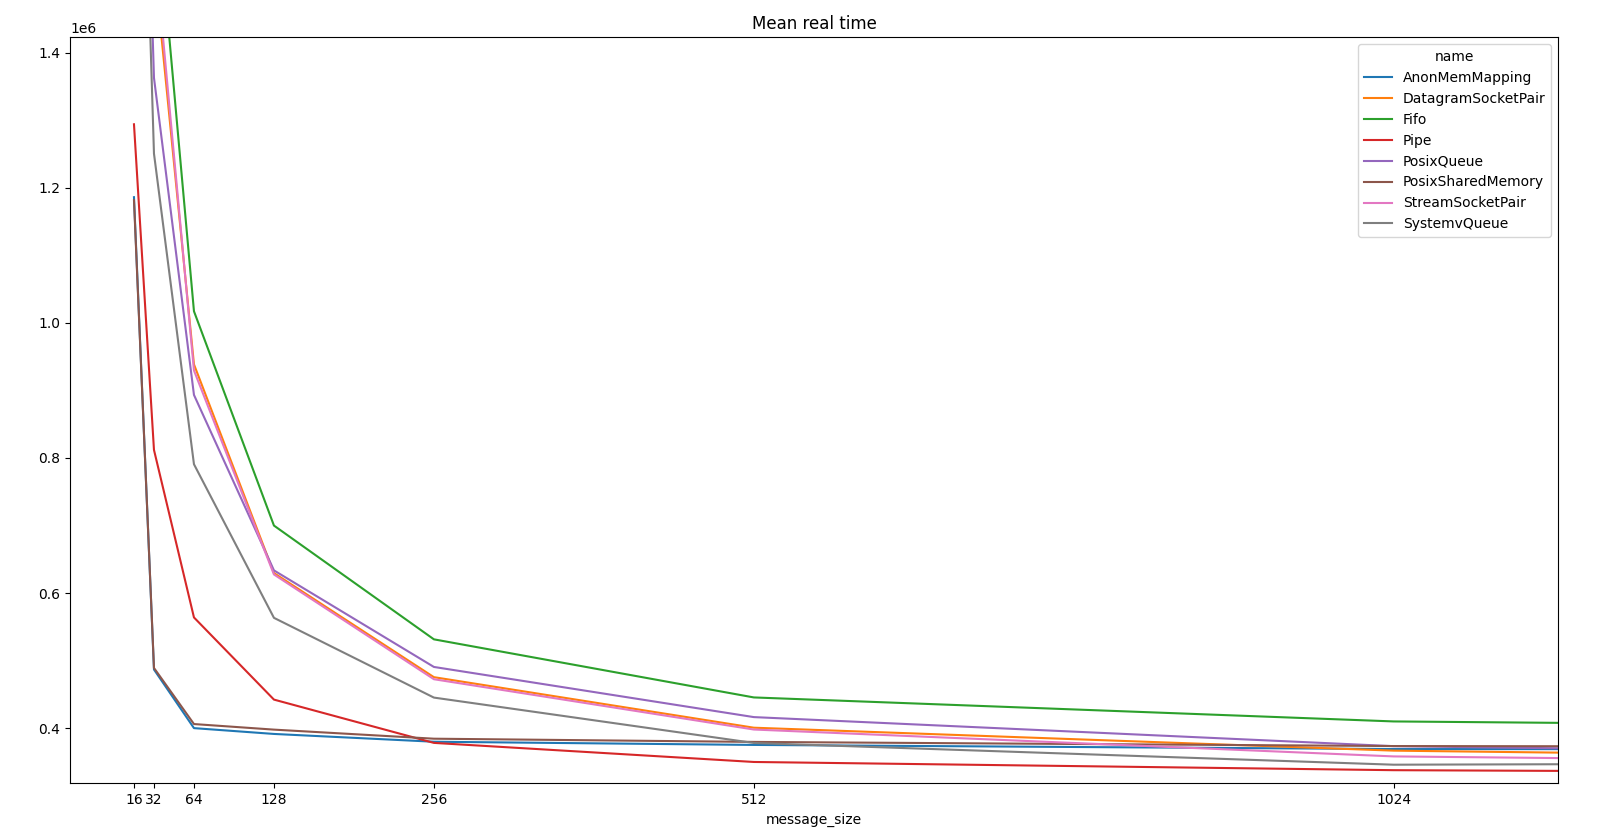
\includegraphics[width=\textwidth]{./imgs/performance.png}
  \end{minipage}
  \caption{Сравнительный график производительности средств межпроцессной
    коммуникации.}
  \label{fig:performance}
\end{figure}

Как и ожидалось, самую высокую производительность для передачи сообщений
небольшого размера показала разделяемая память и анонимная отображаемая память.
Этот отрыв обуславливается экономией на системных вызовах и лишних операциях
копирования в буфер ядра, которые присущи остальным методам межпроцессной
коммуникации.

На больших размерах буферов разницы практически не оказалось, т.к. количество
системных вызовов было сведено к минимуму.

Файловые отображения показали плохие результаты на любом размере буфера, т.к.
зависят от быстродействия персистентной файловой системы. Поэтому они были
намеренно исключены из графика сравнения на этапе подготовки данных.

Стоит упомянуть, что производительность средств межпроцессной коммуникации может
меняться от конкретной конфигурации системы и режима нагрузки, и, например,
зависеть от версии ядра Linux. Измерения приведенные в данной работе выполнены
на версии ядра \verb|6.6.52|, но могут быть легко воспроизведены на любой
целевой системе и гибко сконфигурированны под целевой режим нагрузки путем
изменения размеров и/или количества передаваемых пакетов.

\newpage
\anonsection{ЗАКЛЮЧЕНИЕ}  %Заключение

В ходе выполнения курсовой работы была разработана библиотека для реализации
межпроцессного взаимодействия на базе операционной системы Linux, проведены
тесты производительности интерфейсов данной библиотеки и на их основе оценена
производительность различных механизмов передачи данных между процессами.

Основной целью данной курсовой работы было проведение сравнительного анлиза
средств межпроцессной коммуникации в операцинной системе Linux. Результаты
выполнения задачи демонстрируют корректность реализации библиотеки, на основе
которой реализованы бенчмарки, что подтверждается автоматизированными
юнит-тестами. Разработанные тесты производительности предоставляют гибкий
инструмент для сравнения производительности методов межпроцессной коммуникации в
различных условяих и режимах нагрузки. Были получены и оценены данные о
производительности наиболее релевантных в контексте обмена информацией между
процессами интерфейсов.

В заключение, несмотря на достигнутые положительные результаты, существует
потенциал для дальнейшего улучшения библиотеки. Это включает в себя тестирование
и измерение производительности на основе различных реализаций UNIX систем, а
также расширение интерфейса для двунаправленной коммуникации.

\newpage
\renewcommand\refname{СПИСОК ИСПОЛЬЗОВАННЫХ ИСТОЧНИКОВ}
% Список литературы
\clearpage
\phantomsection
\addcontentsline{toc}{section}{\protect\numberline{}\refname}
%\bibliographystyle{ugost2008s}  %utf8gost71u.bst} %utf8gost705u} %gost2008s}
{\catcode`"\active\def"{\relax}
%\bibliography{biblio} %здесь ничего не меняем, кроме, возможно, имени bib-файла
\printbibliography
}
\newpage
\settocdepth{section}
\anonsection{ПРИЛОЖЕНИЕ А}
\vspace{-30pt}

\begin{listing}[H]
  \caption{Определение класса Subprocess}
  \label{lst:subprocess_declaration}
  \inputminted[style=bw, breaklines, frame=single, fontsize = \footnotesize, linenos=false, xleftmargin = 1.5em]{cpp}{./listings/subprocess_declaration.hpp}
\end{listing}

\begin{listing}[H]
  \caption{Определение методов класса FdBufIn}
  \label{lst:fdbufin_definition}
  \inputminted[style=bw, breaklines, frame=single, fontsize = \footnotesize, linenos=false, xleftmargin = 1.5em]{cpp}{./listings/fdbufin_definition.cpp}
\end{listing}

\begin{listing}[H]
  \caption{Определение методов класса FdBufOut}
  \label{lst:fdbufout_definition}
  \inputminted[style=bw, breaklines, frame=single, fontsize = \footnotesize, linenos=false, xleftmargin = 1.5em]{cpp}{./listings/fdbufout_definition.cpp}
\end{listing}

\begin{listing}[H]
  \caption{Реализация GetSyscallError()}
  \label{lst:errors_definition}
  \begin{minted}[style=bw, breaklines, frame=single, fontsize = \footnotesize, linenos=false, xleftmargin = 1.5em]{cpp}
#include <cerrno>
#include <cstring>
#include <format>

namespace stewkk::ipc {

SyscallError GetSyscallError() {
  auto err = errno;
  return SyscallError(err, std::system_category(), std::format("{}", strerrorname_np(err)));
}

}  // namespace stewkk::ipc
  \end{minted}
\end{listing}

\begin{listing}[H]
  \caption{Объявление класса Pipe}
  \label{lst:pipe_definition}
  \inputminted[style=bw, breaklines, frame=single, fontsize = \footnotesize, linenos=false, xleftmargin = 1.5em]{cpp}{./listings/pipe.hpp}
\end{listing}

\begin{listing}[H]
  \caption{Определение методов класса Pipe}
  \label{lst:pipe_declaration}
  \inputminted[style=bw, breaklines, frame=single, fontsize = \footnotesize, linenos=false, xleftmargin = 1.5em]{cpp}{./listings/pipe.cpp}
\end{listing}

\begin{listing}[H]
  \caption{Скрипт для построения графика результатов бенчмарков}
  \label{lst:plot}
  \inputminted[style=bw, breaklines, frame=single, fontsize = \footnotesize, linenos=false, xleftmargin = 1.5em]{py}{./listings/plot.py}
\end{listing}

\end{document}
